While commuting zones are used by researchers as a convenient measure of local labor markets, they have a number of shortcomings for empirical research that are not regularly discussed in the literature. In this section, we evaluate the sensitivity of commuting zone definitions, focusing on two aspects of the TS1990 methodology. First, we show that there is substantial ambiguity over the choice of when to stop merging the clusters, and that small changes in the chosen cutoff height can affect the number and size of the clusters. Second, we show that if there is uncertainty in the input data, the resulting commuting zone definitions can vary substantially. Overall, this uncertainty and subjectivity in the commuting zone definitions contributes to conventional standard errors understating the true level of uncertainty in the estimates, which we show when we return to this issue with our empirical replication in the next section.

\subsection{Choosing Cluster Height}
\FloatBarrier
One sensitive feature of the methodology used by TS is choosing the cutoff value above which no clusters can form, or the maximum dissimilarity, which determines the number of clusters. \cite{TK1987} describe the algorithm for choosing a cutoff value as follows (see page 15): ``As a rule of thumb, a normalized average distance of 0.98 was considered sufficient distance between sets of counties to treat them as separate [Labor Market Areas].'' The article does not provide an analysis of the sensitivity to changing the cutoff marginally up or down. \cite{TS1996}, in an effort to minimize methodological differences between commuting zones for 1980 and 1990, use the same cutoff with no further evaluation for the 1990 data. In this subsection, we investigate how sensitive the resulting clusters are to the choice of the cutoff value.

\begin{figure}
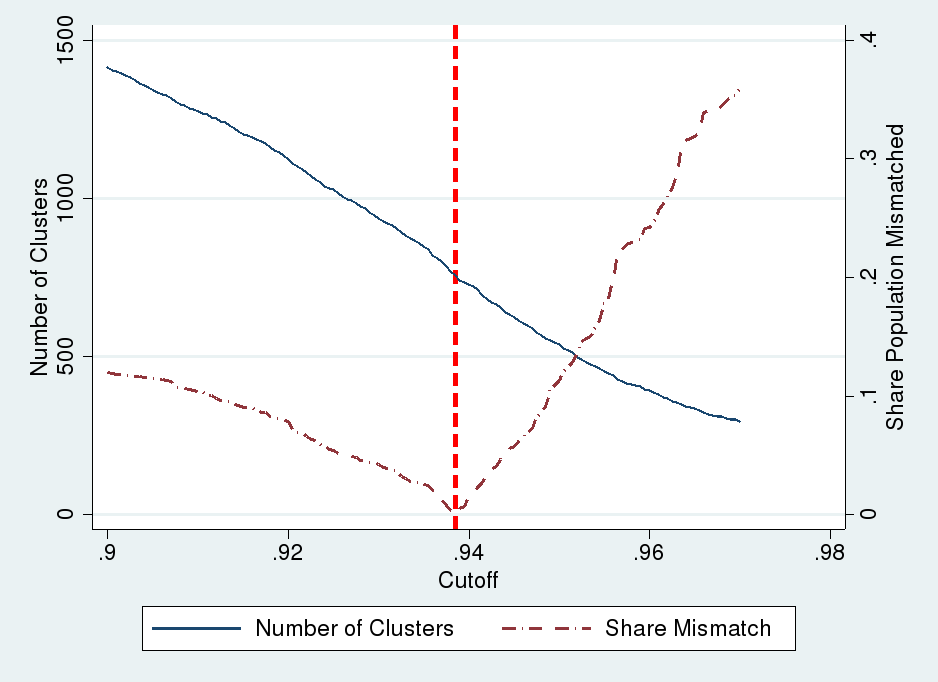
\includegraphics[scale=0.25]{./figures/numclus_cutoff.png}
\caption{Effect of Cluster Height on Number of Clusters \label{fig:cutoff_count}}
\emph{Note:} Authors' calculations using methodology outlined in Section \ref{sec:method}.
\end{figure}

Figure \ref{fig:cutoff_count} shows the number of clusters that form at various height cutoffs using the 1990 JTW data, with the vertical line indicating the cutoff value we chose to replicate TS1990 (0.9385). The key takeaway from this figure is that it is theoretically ambiguous where a researcher should choose to stop merging clusters.\footnote{Decisions on clustering methods, clustering counts, and validation criteria depend on the application and are inherently somewhat subjective. Because clustering is an unsupervised method, there may be no indication of the ideal number of clusters \citep{HBV2001}.} Additionally, increasing or decreasing the cutoff has implications for the number of resulting clusters. Decreasing it to 0.9375 increases the number of clusters by 29, while using a cutoff of 0.93995 cause the number of clusters to decrease by 20. We also graph the share of the population that is in a different cluster than the replicated clusters, to illustrate how assignment changes further away from the cutoff. As we noted earlier, one particular issue with the methodology is that for cutoffs to the right of the vertical line, a large residual cluster forms, which contributes to the steeper slope in the share of the population mismatched.

%As we described above, the measurement error in commuting flows causes some uncertainty in terms of the true dissimilarity matrix, and hence the true cluster heights. Because of the presence of a strict cutoff, some clusters that would have formed if $D_{ij}$ were measured without error do not form, and vis-versa. 

More broadly, TS provide no empirical guidance for choosing the optimal cutoff and cluster size other than referring to expert knowledge. While outside the scope of the current paper, future work may explore data-driven methods to determine whether there is an optimal number of clusters for certain uses. as well as clustering methods that provide more globally optimal clusters.

\subsection{Sensitivity of Clustering Results to Underlying Error}
\FloatBarrier

Another potential sensitivity of the commuting zone methodology is the use of the Journey to Work data, which is subject to sampling error. We analyze the extent to which the outputs of the TS methodology are sensitive to errors in this data. First, recall Equation \ref{eqn:diss} for the entries of the dissimilarity matrix. If $f_{ij}$ is measured without error, then the distance between counties $i$ and $j$ is also measured without error. However, if the flows are measured with error, $\epsilon_{ij}$, then observed flows may be defined as $\hat{f}_{ij}=f_{ij}+\epsilon_{ij}$. In this way, our observed $\hat{rlf}_{i}$, $\hat{rlf}_{j}$, and $\hat{d}_{ij}$ would also include error. We express this assumption below (assuming without loss of generality that $rlf_i < rlf_j$):

\begin{align*}
\hat{d}_{ij} &= 1 - \frac{\hat{f}_{ij} + \hat{f}_{ji}}{\hat{rlf}_i} \\
&= 1- \frac{f_{ij} + f_{ji}}{rlf_{i} + \sum_j \epsilon_{ij}} +  \frac{\epsilon_{ij} + \epsilon_{ji}}{rlf_{i} + \sum_j \epsilon_{ij}}
\end{align*}

Even if $E[\epsilon_{ij}]=0$, that does not imply that $E[\hat{d}_{ij}] = d_{ij}$. Furthermore, we cannot rely on the limit properties of the error distribution, because we only have one realization of the commuting flow, which is calculated from survey responses. Additionally, we know that $\epsilon_{ij}/f_{ij}$ is larger for small flows. Errors will increase $d_{ij}$ for some small counties and decrease it for others. Because of the hierarchical nature of the clustering method, this error will affect the formation of all other clusters in the data.\footnote{Additionally, because heights are normalized in the procedure, it also affects where the effective cutoff is, even for counties unaffected by errors in flows.}

To demonstrate how this measurement error affects the outcome of the clustering procedure, we project the published margins of error (MOE) from the 2009-2013 ACS Journey to Work data onto the 1990 Journey to Work data (which does not publish margins of error). \footnote{To project MOE to 1990, we calculate a ratio, $MOE_{ij}/f_{ij}$, representing the degree of uncertainty for a flow in ACS. To reflect the range of MOEs across similar flows, we calculate the mean and standard deviation of these ratios within flow size bins, defined by 1990 flow percentile, of: 0-50; 50-90; 90-95; 95-99; and 99+. For each 1990 flow, we draw a ratio from the distribution in the corresponding bin. Note that the Census Long form is designed to be a one-in-six sample for one year, while the ACS 5-year summary is designed to 5 years with a one-in-fifty sample each year. The smaller sample size typically results in higher margins of error in the ACS for comparable statistics. The uncertainty implied by our implementation likely overstates the underlying MOEs in the 1990 JTW. For more information on the construction of the ACS MOEs, refer to \url{https://www2.census.gov/programs-surveys/acs/tech_docs/accuracy/MultiyearACSAccuracyofData2013.pdf}, pages 10-12.} Using these estimated MOEs, we then obtain different realizations of the commuting zones in the following way:

\begin{enumerate}
	\item For each origin-destination pair ($i,j$), we draw $\epsilon_{ij}$ from a normal distribution with mean 0 and standard deviation $MOE_{ij}/(1.645)$, since the MOE is scaled to be the 90\% confidence interval.\footnote{In doing this, we assume that $\epsilon_{ij} \perp \epsilon_{ik} \forall k$, for simplicity. In reality, it is likely that $corr(\epsilon_{ij},\epsilon_{ik})<0$, which means in our setting that we are understating the error by treating them as independent. In the JTW data, there are likely some origin-destination pairs that are not reported due to the sample design. In our current resampling approach, we only resample from non-zero flows in the data. A more complete approach would be to model the likelihood that a zero reported is actually a positive flow, and resample accordingly. This modeling is beyond the scope of this paper. For more detail on the 1990 Decennial Census sample design, consult \url{https://www2.census.gov/prod2/decennial/documents/D1-D90-PUMS-14-TECH-01.pdf}.}
	\item Calculate the new flow value, $\hat{f_{ij}} = f_{ij} + \epsilon_{ij}$, with negative values set to zero.\footnote{Many small flows, 65 percent, are not distinguishable from zero and are at risk to be censored, but these tend to be small flows and account for only 1.7 percent of jobs.}
	\item Re-calculate each dissimilarity matrix entry $\hat{d}_{ij}$. 
	\item Re-run the hierarchical clustering procedure, using the same cutoff as the replication.
	\item Store the new clusters, and calculate the following statistics: average number of counties in a cluster; number of clusters; and total number of counties in a different cluster than the one they were originally assigned.
\end{enumerate}

We iterate over this procedure 1000 times in order to obtain distributions for these statistics. These graphs are shown in Figure \ref{fig:sensitivity}, where the red vertical dashed lines are the values for our replication, FKV1990, obtained using the published 1990 data. The figures show that the average cluster size varies considerably from the result the published figures would yield. The share of the population that is mismatched turns out to be less than 1\% of the US population, even in the most varied cases.

\begin{figure}
\caption{Results from Re-sampling Commuting Flows  \label{fig:sensitivity}}
\begin{tabular}{ccc}
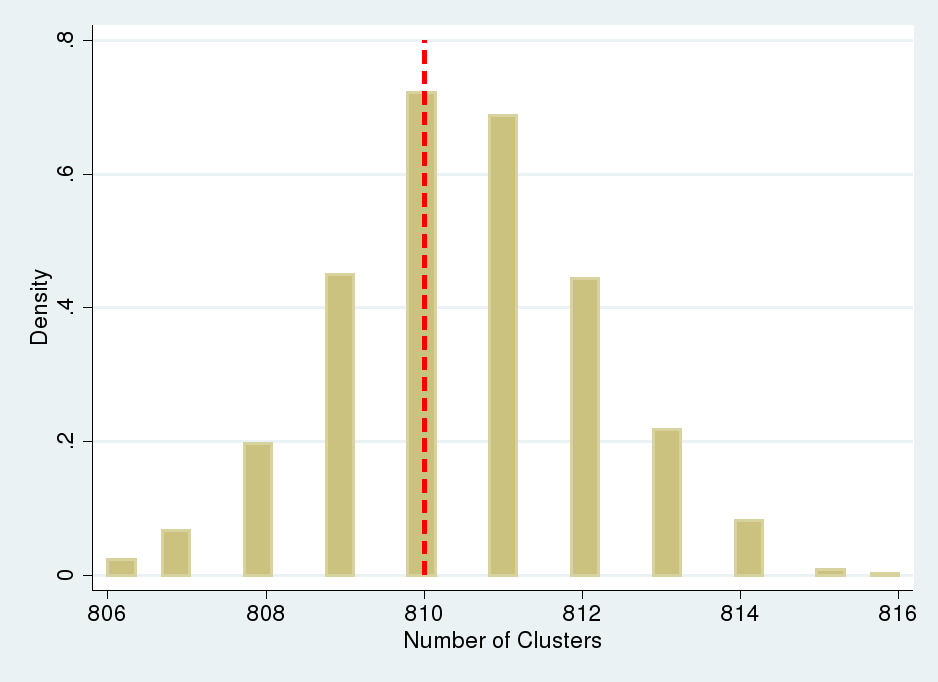
\includegraphics[scale=.15]{./figures/numclusters_jtw1990.png}& 
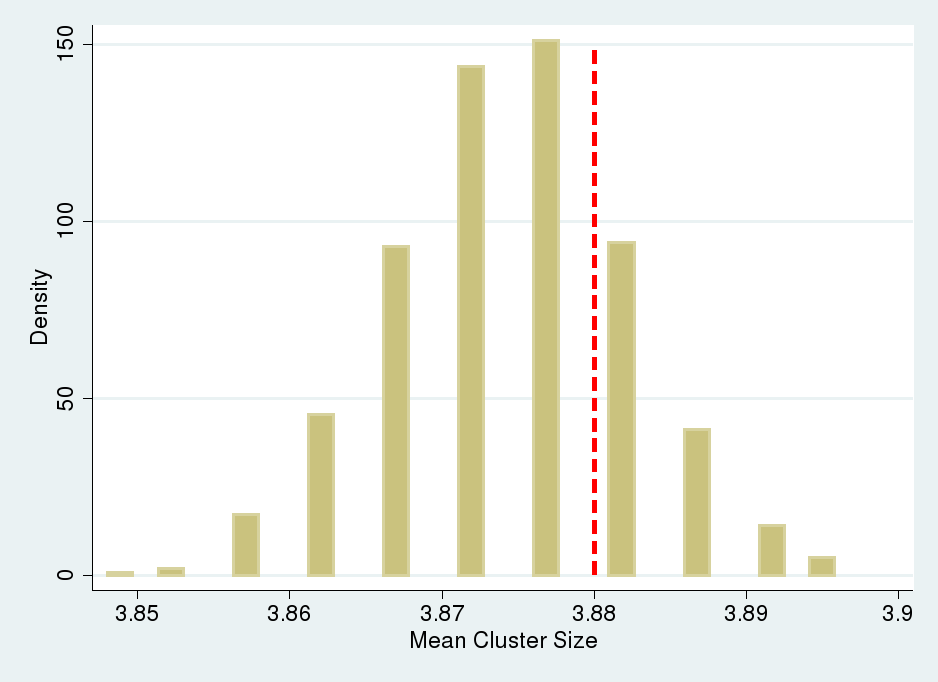
\includegraphics[scale=.15]{./figures/meanclussize_jtw1990.png}&
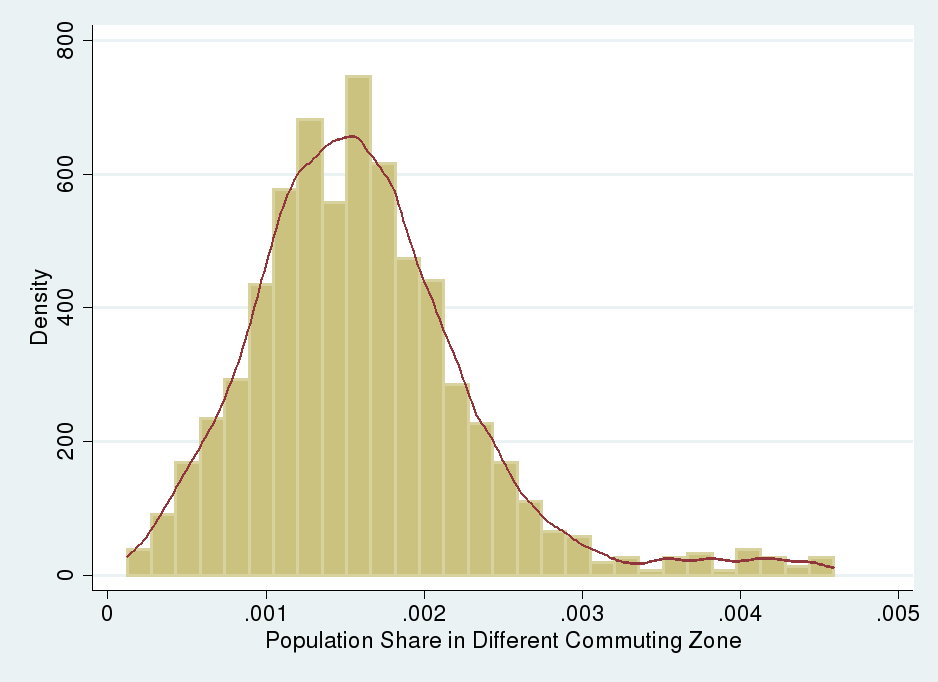
\includegraphics[scale=.15]{./figures/mismatch_jtw1990.png} \\ 
(a) Number of clusters & (b) Average Number of Counties & (c) Share of Mismatched Population \\
\end{tabular}
\end{figure}

